	\section{Gain}
	
	Lets look on avalanche process in the tube. If multiplication occurs, the increasing of the number of electrons per path $ds$ is given by
	
	\begin{equation}
		dN = N \alpha ds
		\label{eq:diffGain}
	\end{equation}
	
	The coefficient $\alpha$ is determined by the excitation and ionization cross sections of the electrons that have acquired sufficient energy in the field. It also depends on the various transfer mechanisms and electric field E and increases with the field because the ionization cross-section goes up from threshold as the collision energy $\varepsilon$ increases. As we can suppose the coefficient $\alpha$ is of big amount of parameters.
	
	The amplification factor $G$ on a wire(that is more interesting for us) is given by integrating (\ref{eq:diffGain}) between the point $s_{min}$ where the field is just sufficient to start the avalanche and the wire radius $a$:
	
	\begin{equation}
	G = N/N_0 = exp \int\limits_{s_{min}}^{a} \alpha(s) ds
	\label{eq:gain}
	\end{equation}
	
	GARFIELD can provide us by amplification factor $G$ for any point of the tube(because  $G$ is coordinate dependent magnitude). The amplification factor is equal almost in whole tube space except neighbourhood near the wire because electric field  becomes significantly high only near the wire (see figs \ref{fig:elFieldCentered}, \ref{fig:elField1mmShifted}). When the wire is shifted from the center of the tube the electric field in area close to the wire is the same as in centered state. So the amplification factor $G$ is quite similar in both cases.
	
	\begin{figure}[!h] 
		\centering
		\subfloat[electric field for centered wire]{
			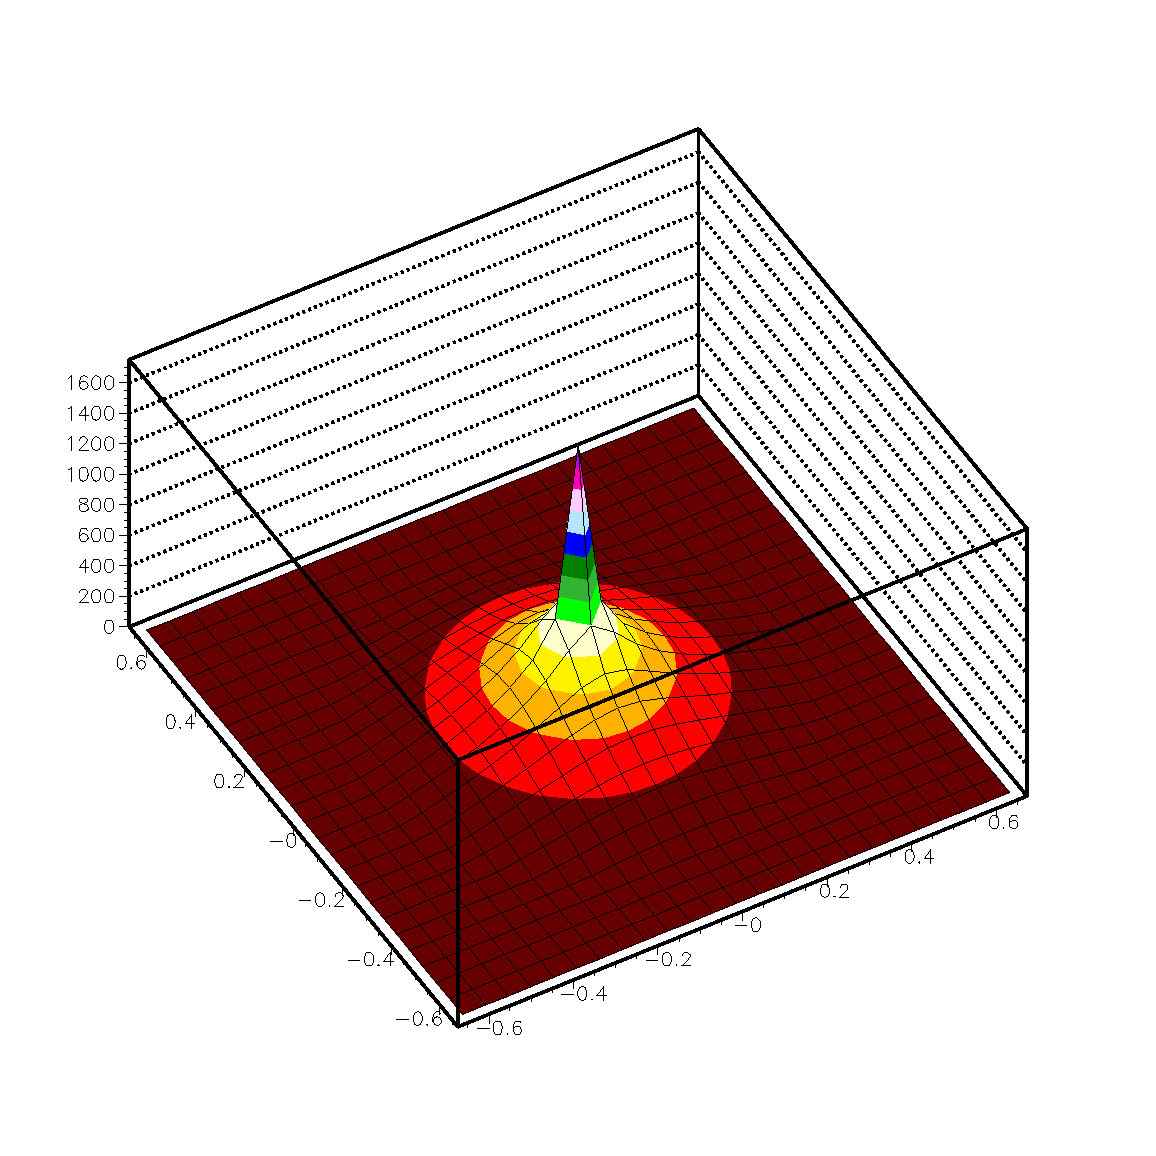
\includegraphics[width=0.45\textwidth]{fieldCentered} 
			\label{fig:elFieldCentered} }%
		\qquad
		\subfloat[electric field for $1 mm$ shifted wire]{
			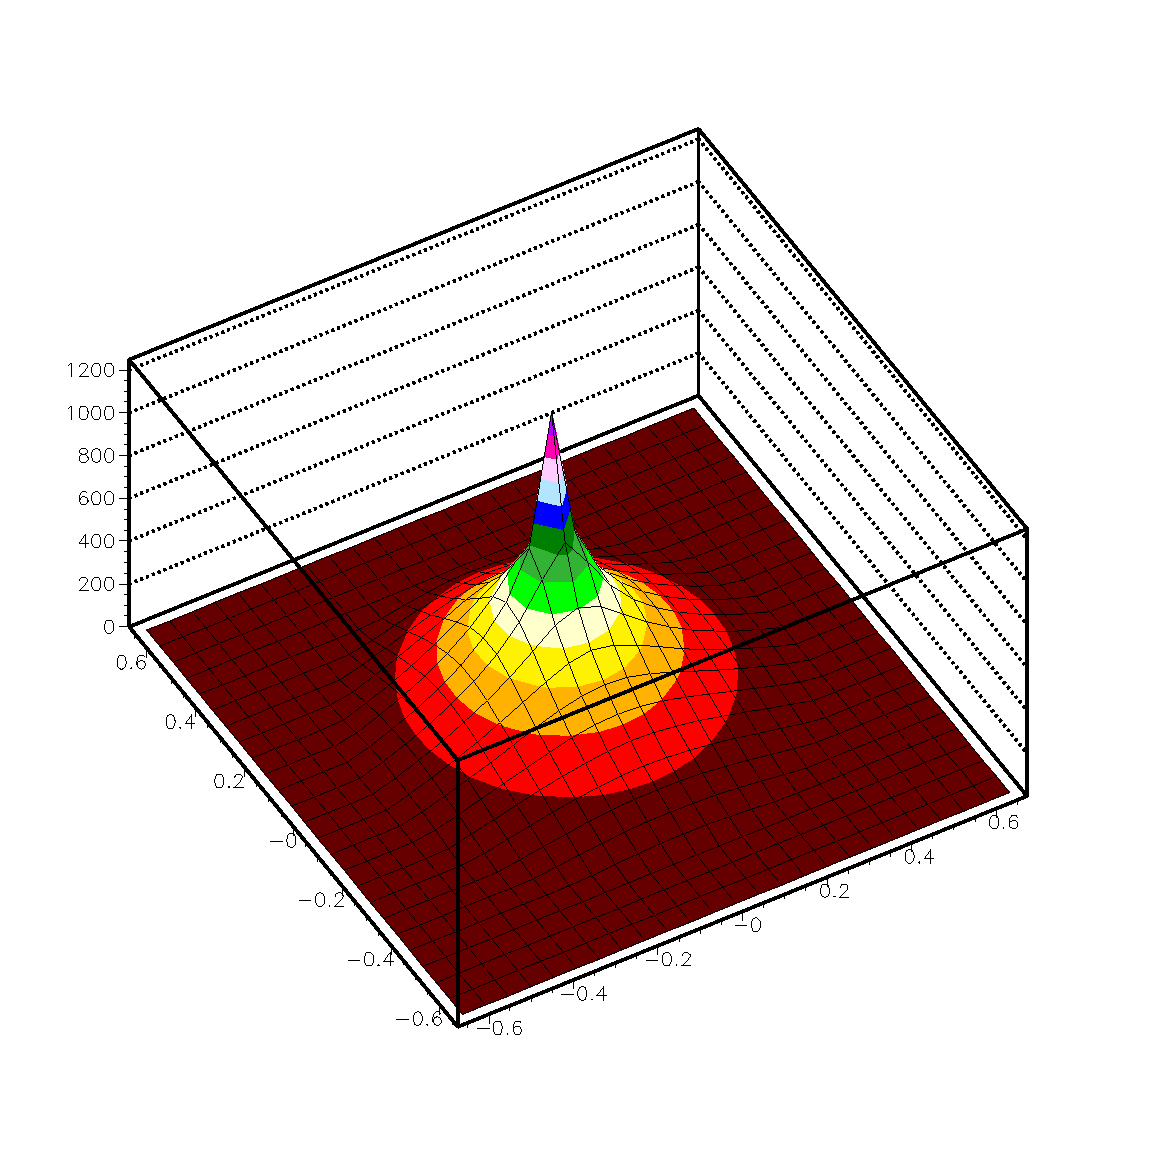
\includegraphics[width=0.45\textwidth]{field_10Sag}
			\label{fig:elField1mmShifted} }%
		\caption{Electric field intensity map for different wire position in the cube calculated in GARFIELD software. Conditions for those plots are described in table \ref{table:straw_par} }
	\end{figure}
	
	Implementation of gain value calculation is not so reliable in GARFIELD(especially fortran version). Gain should be recalculated using Garfield++ (which is newer and takes into consideration more effects). 
	
	\begin{figure}[h!]
	\centering
	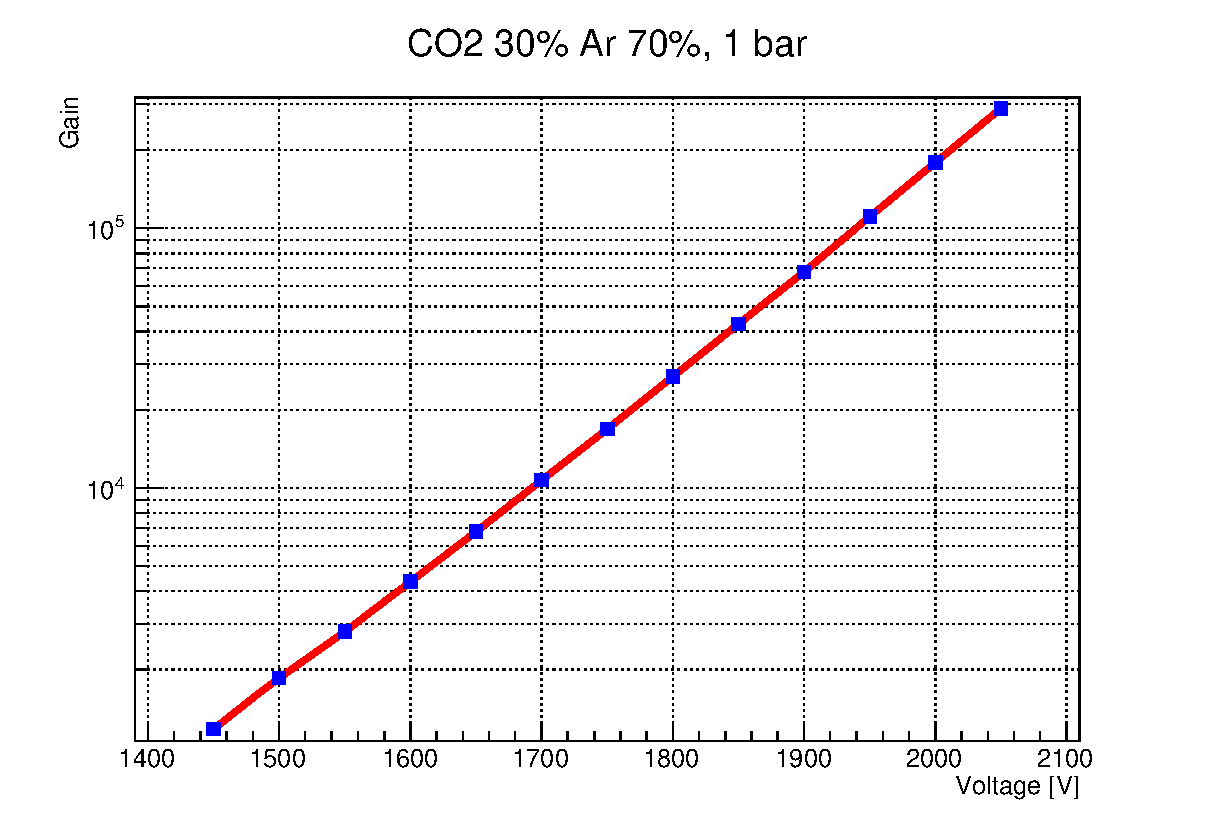
\includegraphics[width=0.7\textwidth]{gain_1450_2050V}	
	\caption{Dependence of the gain of the voltage applied to the wire. The rest of STRAW tube settings corresponds to table \ref{table:straw_par}. }
	\label{fig:gainVoltage}	
	\end{figure}

	On the Fig.\ref{fig:gainVoltage} you can see that the gain $G(V)$ have precisely exponential dependence. This is frankly does not inspire confidence. The difference can be up to 100\% (as Rob Veenhof - creator of GARFIELD \cite{garfield} said).
	